\chapter{Contesto scientifico e fondamenti teorici}
\label{chap:fondamenti}

Per descrivere il confronto tra reti classiche e ibride occorre partire
dall'informazione contenuta nelle immagini e dal modo in cui viene
rappresentata. Il capitolo introduce le categorie morfologiche, il
transfer learning e le operazioni quantistiche utilizzate nel modello.
La costruzione del campione e le scelte sperimentali sono trattate
separatamente nei \cref{chap:dataset,chap:modelli}.

\section{Classificazione morfologica delle galassie}
\label{sec:fond-morfologia}

\subsection{Informazione morfologica e classi considerate}

La morfologia descrive l'aspetto e l'organizzazione delle strutture visibili
di una galassia. Il suo studio contribuisce a caratterizzare le popolazioni
galattiche e a indagarne formazione ed evoluzione. La classificazione da
immagini riguarda però una proiezione osservata del sistema, non una
ricostruzione completa delle sue proprietà fisiche.

Nel contesto della tesi si considerano tre categorie operative. Le galassie
\emph{ellittiche} presentano generalmente una distribuzione della luminosità
relativamente regolare, senza bracci a spirale chiaramente riconoscibili.
Le \emph{spirali} mostrano una struttura a disco nella quale possono essere
visibili bracci e una componente centrale. L'aspetto osservato dipende
anche dall'orientamento: una galassia a disco vista di taglio non mostra
i bracci nello stesso modo di una vista frontalmente.

La categoria \emph{merger} identifica invece sistemi classificati come
associati a un'interazione o fusione, che possono mostrare componenti
multiple, asimmetrie e strutture perturbate. Non si tratta di una categoria
morfologica equivalente, sul piano fisico, a ellittica o spirale:
l'interazione è un processo che può coinvolgere galassie di morfologie
diverse. Il lavoro di Darg et al.~\cite{darg2010mergers} illustra l'impiego
delle classificazioni Galaxy Zoo per studiare questi sistemi. Nella tesi
merger è una classe definita dalle regole di selezione del catalogo, non
una diagnosi fisica ricavata autonomamente dal classificatore.

\begin{figure}[tbp]
\centering
\begin{minipage}{0.31\textwidth}
\centering
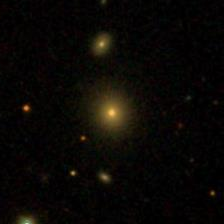
\includegraphics[width=\linewidth]{figures/foundations/elliptical.png}\\
\small (a) Ellittica
\end{minipage}\hfill
\begin{minipage}{0.31\textwidth}
\centering
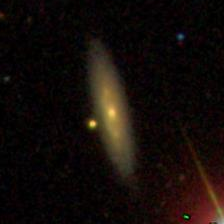
\includegraphics[width=\linewidth]{figures/foundations/spiral.png}\\
\small (b) Spirale
\end{minipage}\hfill
\begin{minipage}{0.31\textwidth}
\centering
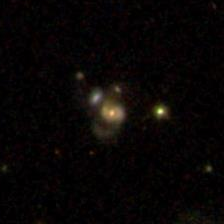
\includegraphics[width=\linewidth]{figures/foundations/merger.png}\\
\small (c) Sistema etichettato merger
\end{minipage}
\caption{Esempi reali del dataset derivato da immagini SDSS e classificazioni
Galaxy Zoo. Sono mostrati ritagli centrali di \(224\times224\) pixel,
senza sovrapposizioni interpretative. Gli identificativi degli oggetti sono,
da sinistra, \texttt{1237656241699881339}, \texttt{1237651273507668077} e
\texttt{1237655499209310435}. Gli esempi sono illustrativi, non prototipi
esaustivi delle classi; l'etichetta merger non costituisce da sola una
conferma fisica di fusione.}
\label{fig:fond-esempi}
\end{figure}

\subsection{Survey, annotazioni e difficoltà del riconoscimento}

Le survey astronomiche producono raccolte di immagini per le quali
l'ispezione individuale non è facilmente scalabile. Galaxy Zoo ha affrontato
il problema coinvolgendo volontari nella classificazione delle immagini
SDSS; il rilascio Galaxy Zoo 1 rende disponibili classificazioni
morfologiche aggregate per un ampio campione di galassie
\cite{lintott2011galaxyzoo}. Le frazioni di voto descrivono le risposte
dei classificatori e il loro accordo: non vanno identificate automaticamente
con probabilità fisiche certe di appartenenza a una classe.

Risoluzione, rapporto segnale-rumore, orientamento e presenza di sorgenti
vicine influenzano ciò che è riconoscibile nell'immagine. Inoltre, una
distribuzione luminosa perturbata può essere più difficile da descrivere
con una singola etichetta. Ciò motiva l'uso della classe merger come
ulteriore banco di prova, senza assumere a priori che essa debba essere
sempre la più difficile per qualsiasi modello.

Il passaggio da due a tre classi modifica sia le decisioni richieste sia
la composizione del problema. Non equivale a modificare un solo parametro
di difficoltà mantenendo invariato tutto il resto. Soglie di voto,
bilanciamento e separazione degli oggetti tra training e test devono
quindi essere esplicitati, come avviene nel \cref{chap:dataset}.

\section{Apprendimento profondo e transfer learning}
\label{sec:fond-transfer}

\subsection{Reti convoluzionali e rappresentazioni delle immagini}

Una rete convoluzionale elabora un'immagine mediante filtri applicati a
regioni locali, condividendo gli stessi pesi tra posizioni diverse.
Le uscite sono mappe di attivazione: ciascun canale risponde a determinati
pattern appresi durante l'addestramento. La composizione di strati
convoluzionali e trasformazioni non lineari consente di combinare
informazioni locali in rappresentazioni progressivamente più elaborate.

Non è necessario definire manualmente una misura per ogni possibile
struttura morfologica. Tuttavia, non è neppure corretto attribuire
automaticamente a ogni attivazione un significato astronomico preciso:
una feature appresa può mescolare forma, colore, tessitura e informazioni
legate al processo osservativo. L'impiego delle CNN nella classificazione
galattica è esemplificato da Dieleman et al.~\cite{dieleman2015galaxy},
che incorporano le simmetrie delle immagini nel modello di riconoscimento.

Una distinzione utile è quella tra \emph{estrattore di feature}, che
trasforma l'immagine in una rappresentazione, e \emph{testa di
classificazione}, che usa tale rappresentazione per produrre i punteggi
delle classi. Questa separazione permette di studiare teste diverse
senza modificare ogni volta l'intero sistema di visione.

\subsection{Reti residuali e ResNet18}

Le reti residuali introducono collegamenti che sommano l'ingresso di
un blocco alla trasformazione appresa dal blocco stesso
\cite{he2016resnet}. Quando le dimensioni coincidono, il principio è
espresso da
\begin{equation}
 \boldsymbol y=F(\boldsymbol x;\boldsymbol w)+\boldsymbol x.
\end{equation}
Il blocco apprende così una correzione rispetto alla rappresentazione
in ingresso. Quando cambiano le dimensioni, il collegamento può includere
una proiezione. Queste connessioni facilitano l'ottimizzazione di reti
profonde, senza garantire da sole una migliore generalizzazione per
qualunque dataset.

ResNet18 è una variante relativamente compatta della famiglia. Eliminando
il classificatore finale si ottiene, dopo l'aggregazione spaziale delle
mappe, un vettore di 512 componenti. Nel presente lavoro questa
rappresentazione costituisce il punto di partenza comune dei modelli.
Il numero 512 indica la dimensione del vettore, non un elenco di 512
proprietà fisiche delle galassie note a priori.

\subsection{Preaddestramento, congelamento e fine-tuning}

Il transfer learning riutilizza una rappresentazione appresa su un
problema sorgente per affrontarne un altro. È possibile aggiornare
anche i pesi dell'estrattore sul nuovo dataset, effettuando
\emph{fine-tuning}, oppure mantenerli fissi e addestrare soltanto la testa.
La seconda strategia riduce il numero di parametri da stimare e consente
di riutilizzare le feature già calcolate.

Il riuso di feature apprese su immagini naturali non implica che esse
siano ottimali per immagini astronomiche. È una scelta sperimentale
che introduce un limite, ma permette anche un confronto più controllato:
le differenze tra teste non dipendono da backbone addestrati separatamente.
Nel presente lavoro ResNet18 è preaddestrata su ImageNet e congelata; il
trasferimento al dominio galattico avviene attraverso gli strati successivi.
Di conseguenza, la componente quantistica riceve feature classiche
compresse, non direttamente i pixel dell'immagine.

\section{Fondamenti di calcolo quantistico}
\label{sec:fond-quantum}

Si richiamano qui le nozioni del modello a circuito necessarie per
leggere l'architettura ibrida. Per una trattazione sistematica di stati,
porte e misure si rimanda a Nielsen e Chuang~\cite{nielsen2010quantum}.

\subsection{Qubit e registri quantistici}

Un qubit è descritto, nel caso di uno stato puro, da un vettore normalizzato
in uno spazio complesso bidimensionale:
\begin{equation}
 |\psi\rangle=\alpha|0\rangle+\beta|1\rangle,
 \qquad \alpha,\beta\in\mathbb C,
 \qquad |\alpha|^2+|\beta|^2=1.
\end{equation}
I vettori \(|0\rangle\) e \(|1\rangle\) formano la base computazionale.
Una misura in questa base restituisce 0 oppure 1, con probabilità
rispettivamente \(|\alpha|^2\) e \(|\beta|^2\). La sovrapposizione
descrive lo stato prima della misura: non significa poter leggere
simultaneamente entrambi i valori come due bit classici.

Per \(q\) qubit lo spazio degli stati è il prodotto tensoriale degli
spazi dei singoli qubit e ha dimensione \(2^q\). Uno stato puro generale è
\begin{equation}
 |\psi\rangle=\sum_{z=0}^{2^q-1}c_z|z\rangle,
 \qquad \sum_z|c_z|^2=1.
\end{equation}
La crescita dello spazio delle ampiezze è importante, ma non dimostra
un vantaggio nell'apprendimento: preparazione dello stato, trasformazioni
realizzabili e modalità di lettura limitano l'informazione accessibile.

\subsection{Porte, rotazioni ed entanglement}

Nel modello ideale a circuito, le porte trasformano lo stato mediante
operatori unitari. Le rotazioni impiegate in questa tesi sono
\begin{equation}
 R_Y(a)=
 \begin{pmatrix}\cos(a/2)&-\sin(a/2)\\
 \sin(a/2)&\cos(a/2)\end{pmatrix},
 \qquad
 R_Z(b)=
 \begin{pmatrix}e^{-ib/2}&0\\0&e^{ib/2}\end{pmatrix}.
\end{equation}
Applicata a \(|0\rangle\), la prima produce
\(\cos(a/2)|0\rangle+\sin(a/2)|1\rangle\): un angolo classico
controlla quindi le ampiezze dello stato. La seconda agisce sulle fasi;
il suo effetto sulle probabilità osservate dipende anche dalle operazioni
successive, che possono convertire differenze di fase in differenze
misurabili.

La porta CNOT coinvolge un qubit di controllo e uno bersaglio:
\begin{equation}
 \operatorname{CNOT}|c,t\rangle=|c,t\oplus c\rangle,
 \qquad c,t\in\{0,1\},
\end{equation}
dove \(\oplus\) è la somma modulo due. Su opportune sovrapposizioni
può generare entanglement. Per uno stato puro, questo significa che lo
stato congiunto non è esprimibile come prodotto degli stati dei singoli
sottosistemi. La presenza di una CNOT non garantisce però che ogni input
generi uno stato entangled, né che tali correlazioni migliorino la
classificazione.

\subsection{Misure e valori attesi}

Per usare il circuito in un classificatore occorre ottenere uscite
numeriche. La misura dell'osservabile di Pauli
\(Z=\operatorname{diag}(1,-1)\) ha esiti \(+1\) e \(-1\). Il suo
valore atteso sul qubit \(i\) è
\begin{equation}
 z_i=\langle\psi|Z_i|\psi\rangle
     =P_i(0)-P_i(1),\qquad z_i\in[-1,1],
\end{equation}
dove \(Z_i\) agisce sul qubit considerato e come identità sugli altri.
Leggendo un'osservabile per qubit si ottiene un vettore reale di
dimensione \(q\), senza ricostruire tutte le \(2^q\) ampiezze.

Su hardware, un valore atteso è normalmente stimato ripetendo preparazione
e misura per un numero finito di esecuzioni, dette \emph{shot}. Una
simulazione ideale dello stato può invece calcolarlo direttamente, senza
rumore di campionamento delle misure. Questa distinzione è essenziale
per interpretare sia il training sia i costi.

\section{Reti neurali ibride classico-quantistiche}
\label{sec:fond-ibrido}

\subsection{Encoding delle feature}

Un circuito destinato a elaborare dati classici richiede una mappa di
codifica. Nell'\emph{angle encoding} le componenti di un vettore
determinano gli angoli delle porte. Per esempio,
\begin{equation}
 |\phi(\boldsymbol a)\rangle=
 \left[\bigotimes_{i=1}^{q}R_Y(a_i)\right]|0\rangle^{\otimes q}.
\end{equation}
La codifica non assegna una classe a ciascun qubit: tutti i valori in
uscita possono contribuire alla decisione su ciascuna classe.

Quando le feature iniziali sono più numerose dei qubit, una trasformazione
classica può comprimerle e limitarne l'intervallo prima dell'encoding.
Questa proiezione è parte del modello e può essere addestrabile.
La rappresentazione risultante va distinta dall'\emph{amplitude encoding},
nel quale i dati sono codificati nelle ampiezze di uno stato normalizzato.
Le strategie comportano operazioni e costi diversi e non sono
intercambiabili senza modificare il modello.

Un'altra distinzione riguarda il \emph{data re-uploading}, che inserisce
nuovamente i dati in più punti del circuito. Il circuito principale
della tesi usa invece un solo blocco iniziale di encoding; la ripetizione
degli strati parametrizzati non equivale a ripetere la codifica dei dati.

\subsection{Circuiti variazionali e architettura ibrida}

Un circuito variazionale applica una trasformazione
\(U(\boldsymbol\theta)\) con parametri regolabili. La disposizione
delle porte e dei collegamenti, detta \emph{ansatz}, definisce la famiglia
di trasformazioni esplorata durante il training. È utile distinguere
gli angoli \(\boldsymbol a\), che dipendono dall'esempio, dai pesi
\(\boldsymbol\theta\), condivisi tra gli esempi e aggiornati
dall'ottimizzatore.

Nel paradigma ibrido una rete classica prepara gli ingressi del circuito
e una seconda trasformazione ne elabora le letture. Mari et al.
\cite{mari2020transfer} formalizzano questo schema nel contesto del
transfer learning. Una scrittura generale è
\begin{equation}
 \boldsymbol\ell(x)=h_{\boldsymbol\omega}
 \left(\boldsymbol z_{\boldsymbol\theta}
 \left(g_{\boldsymbol\eta}(F_{\mathrm{pre}}(x))\right)\right),
\end{equation}
dove \(F_{\mathrm{pre}}\) è l'estrattore preaddestrato,
\(g_{\boldsymbol\eta}\) la proiezione classica,
\(\boldsymbol z_{\boldsymbol\theta}\) il vettore dei valori attesi e
\(h_{\boldsymbol\omega}\) la testa finale. Le componenti di
\(\boldsymbol\ell\) sono punteggi, detti \emph{logit}, convertibili
in probabilità mediante softmax. Le letture quantistiche non sono
quindi, da sole, probabilità delle classi.

\begin{figure}[tbp]
\centering
\resizebox{\textwidth}{!}{% Schema originale: solo TikZ e arrows.meta, gia' nel preambolo.
\begin{tikzpicture}[
 box/.style={draw=black!55,rounded corners=2pt,align=center,
 text width=2.15cm,minimum height=1cm,font=\small,inner sep=5pt},
 flow/.style={-{Latex[length=2mm]},draw=black!65,thick}]
\node[box,fill=black!3] (image) at (0,0) {Immagine\\\(x\)};
\node[box,fill=black!3] (backbone) at (3.1,0)
 {Estrattore classico\\congelato};
\node[box,fill=blue!5] (pre) at (6.2,0)
 {Proiezione\\\(\boldsymbol a=g_{\boldsymbol\eta}(\boldsymbol f)\)};
\node[box,fill=violet!8] (quantum) at (9.3,0)
 {Blocco quantistico\\\(\boldsymbol z_{\boldsymbol\theta}(\boldsymbol a)\)};
\node[box,fill=blue!5] (head) at (12.4,0)
 {Classificatore\\logit di classe};
\draw[flow] (image) -- (backbone);
\draw[flow] (backbone) -- node[above,font=\small]{\(\boldsymbol f\)} (pre);
\draw[flow] (pre) -- (quantum);
\draw[flow] (quantum) -- (head);
\node[box,fill=violet!3] (encode) at (6.2,-2.1)
 {Encoding\\\(R_Y(a_i)\)};
\node[box,fill=violet!8] (unitary) at (9.3,-2.1)
 {Trasformazione\\\(U(\boldsymbol\theta)\)};
\node[box,fill=violet!3] (readout) at (12.4,-2.1)
 {Lettura\\\(\langle Z_1\rangle,\ldots,\langle Z_q\rangle\)};
\draw[flow] (encode) -- (unitary);
\draw[flow] (unitary) -- (readout);
\draw[dashed,draw=black!40] (quantum.south) -- (unitary.north);
\node[align=left,font=\small,text width=3.8cm] at (1.1,-2.1)
 {Dettaglio funzionale\\del blocco quantistico};
\end{tikzpicture}
}
\caption{Schema concettuale di un classificatore ibrido con estrattore
congelato. Il dettaglio inferiore distingue encoding dipendente dai dati,
trasformazione variazionale e lettura. Si tratta di uno schema funzionale,
non del circuito specifico implementato, descritto nel \cref{chap:modelli}.}
\label{fig:fond-ibrido}
\end{figure}

\subsection{Addestramento e circuito congelato}

La funzione di perdita confronta le predizioni con le etichette e guida
l'aggiornamento dei parametri addestrabili. Per ottimizzare la proiezione
classica occorre derivare la perdita anche rispetto agli ingressi del
circuito. La catena di derivate collega quindi componenti classiche e
quantistiche; non si tratta di addestrare due classificatori indipendenti.

Su simulatori differenziabili è possibile usare la differenziazione
automatica. Su hardware, per opportune porte parametrizzate, regole come
il \emph{parameter-shift} permettono di ricavare derivate da valutazioni
del circuito con parametri traslati \cite{schuld2019gradients}. Le due
modalità non hanno lo stesso costo operativo; quella effettivamente
adottata è precisata nel \cref{chap:modelli}.

Congelare \(\boldsymbol\theta\) lascia invece fissa la trasformazione
circuitale. Il modello può continuare ad apprendere attraverso
\(\boldsymbol\eta\) e \(\boldsymbol\omega\), e le uscite del circuito
continuano a cambiare al cambiare dell'input. Questo controllo consente
di distinguere il contributo dell'inserimento del circuito da quello
dell'ottimizzazione dei suoi pesi.

\subsection{Simulazione e processori quantistici}

La simulazione classica consente di valutare il comportamento matematico
di un circuito, ma non ne riproduce necessariamente il costo su un
processore quantistico. Una simulazione generica a vettore di stato
memorizza \(2^q\) ampiezze complesse; il costo dipende anche dal numero
e dal tipo di porte, dal batch e dal metodo di differenziazione.
Non si può quindi attribuire ogni differenza temporale al solo numero
di parametri addestrabili.

In questa tesi le operazioni quantistiche sono simulate e i valori attesi
sono calcolati senza shot finiti. Non si modellano rumore del dispositivo,
errori di lettura o vincoli di accesso a una QPU. L'esperimento studia
il comportamento predittivo delle architetture e il costo della loro
implementazione simulata, non un'accelerazione ottenuta su hardware
quantistico.

\section{Potenzialità, limiti e criteri di confronto}
\label{sec:fond-confronto}

\subsection{Espressività, generalizzazione e ottimizzazione}

L'espressività riguarda le funzioni rappresentabili da un modello;
la generalizzazione riguarda le prestazioni su esempi non usati per
addestrarlo. Una famiglia più ampia non garantisce una generalizzazione
migliore: contano dati disponibili, regolarizzazione e procedura di
ottimizzazione. Anche un numero ridotto di pesi non implica automaticamente
un vantaggio nei regimi con pochi esempi.

Per i circuiti quantistici, McClean et al.~\cite{mcclean2018barren}
mostrano che determinate famiglie di circuiti e condizioni di
inizializzazione possono produrre gradienti la cui varianza si riduce
esponenzialmente con il numero di qubit. Queste regioni del paesaggio di
ottimizzazione sono dette \emph{barren plateau}. Il fenomeno costituisce
un limite teorico importante, ma non è una spiegazione automatica di
ogni risultato negativo. Non è sufficiente osservare una Macro-F1 bassa
per diagnosticarlo, soprattutto in circuiti piccoli e poco profondi:
servono analisi specifiche dei gradienti e delle condizioni teoriche.

\subsection{Baseline, ablazioni e significato del vantaggio}

Un modello ibrido deve essere confrontato con controlli che permettano
di distinguere l'effetto del circuito da quello di altre scelte. Una
baseline lineare descrive quanto le classi siano linearmente separabili
nello spazio delle feature; una
testa non lineare offre un riferimento più flessibile; un bottleneck
classico della stessa dimensione controlla la compressione. Un'ablazione
con circuito congelato verifica invece il contributo
dell'addestramento dei parametri quantistici.

Capacità comparabile non significa equivalenza delle famiglie funzionali.
Condividere dimensioni e inizializzazioni di alcuni strati riduce le
differenze non pertinenti alla domanda di ricerca, ma non rende i modelli
identici per espressività o ottimizzabilità. Bowles et al.
\cite{bowles2024benchmarking} sottolineano l'importanza delle baseline
e del disegno sperimentale nel valutare modelli di quantum machine
learning, mostrando quanto sia limitante una lettura basata sulla sola
graduatoria delle prestazioni.

Un \emph{vantaggio predittivo} richiede un miglioramento valutato su dati
non usati per selezionare il modello e rispetto a riferimenti adeguati.
Un \emph{vantaggio computazionale} riguarda invece risorse e costi
necessari per ottenere un risultato comparabile. Le due nozioni non
coincidono. Per questo la tesi considera congiuntamente classificazione,
qualità delle probabilità e tempi, con le metriche e gli indicatori
statistici definiti nel \cref{chap:modelli}. La prestazione di un singolo
seed non è sufficiente a caratterizzare un'architettura.

\section{Lavori correlati e posizionamento della tesi}
\label{sec:fond-correlati}

\subsection{Dalla classificazione visuale alle reti profonde}

Galaxy Zoo fornisce un collegamento tra annotazione visuale e analisi
automatica, rendendo disponibili etichette aggregate per immagini
astronomiche \cite{lintott2011galaxyzoo}. Dieleman et al.
\cite{dieleman2015galaxy} mostrano come reti convoluzionali progettate
tenendo conto delle rotazioni possano apprendere la classificazione
morfologica dalle annotazioni. Il loro problema di predizione e la
struttura delle etichette non coincidono però con le tre classi operative
della presente tesi: i punteggi non costituiscono un confronto numerico
diretto con i nostri risultati.

In questo lavoro il backbone preaddestrato rimane fisso. L'analisi si
concentra sulla testa e sulla trasformazione applicata alle feature
compresse, mantenendo comune la rappresentazione fornita ai modelli.

\subsection{Transfer learning classico-quantistico}

Mari et al.~\cite{mari2020transfer} costituiscono il riferimento
architetturale per combinare un estrattore classico preaddestrato con
un circuito variazionale e strati classici di interfaccia. L'interesse
è rendere utilizzabili piccoli registri quantistici su rappresentazioni
di immagini ad alta dimensionalità. Questa fattibilità non implica,
da sola, che il circuito superi una testa classica ben controllata.

Otgonbaatar et al.~\cite{otgonbaatar2023transfer} studiano il transfer
learning quantistico su dataset reali di telerilevamento, anche piccoli
e ad alta dimensionalità. Il contesto motiva l'attenzione alla scarsità
di dati, ma non consente di trasferire direttamente conclusioni al
dominio galattico. Differiscono caratteristiche delle immagini,
etichette e configurazioni circuitali.

Kim et al.~\cite{kim2023transfer} considerano invece il trasferimento
verso reti convoluzionali quantistiche. È importante distinguere questa
impostazione dalla nostra: nel presente studio convoluzioni ed estrazione
spaziale rimangono classiche; il circuito interviene soltanto sul vettore
di feature compresso. L'espressione rete ibrida non identifica quindi
un'unica architettura.

\subsection{Contributo sperimentale del lavoro}

Il lavoro si colloca tra queste proposte architetturali e l'esigenza di
una valutazione controllata. Lo studio di Bowles et al.
\cite{bowles2024benchmarking} offre un riferimento metodologico per
interrogare il ruolo effettivo delle componenti quantistiche. Anche
in questo caso task e modelli differiscono: non si usa il risultato
di altri benchmark per anticipare l'esito del nostro esperimento.

La tesi studia una rappresentazione classica comune, controlli con
bottleneck di pari dimensione e circuiti sia addestrabili sia congelati.
Il confronto è ripetuto su due task e su diversi regimi di disponibilità
del training, distinguendo evidenze principali e analisi esplorative.
L'obiettivo non è assumere un vantaggio quantistico, ma individuare
se e in quali condizioni il circuito apporti un beneficio rispetto
alle alternative classiche e a quale costo. I capitoli successivi
traducono questa domanda in un dataset verificabile e in un protocollo
sperimentale riproducibile.
